\documentclass{beamer}
\usepackage[T1]{fontenc}
\usepackage{bookman}
\usetheme[numbering=fraction, block=fill]{metropolis}  %source : https://fr.overleaf.com/latex/templates/metropolis-beamer-theme/qzyvdhrntfmr et https://mirror.foobar.to/CTAN/macros/latex/contrib/beamer-contrib/themes/metropolis/doc/metropolistheme.pdf

\usepackage[french]{babel}
\usepackage{enumitem}
\usepackage{booktabs}  % pour toprule, etc
\usepackage{amsfonts}
\usepackage{amsmath}
\usepackage{amssymb}
\usepackage{amsthm}
\usepackage{hyperref}%   liens internet
\usepackage{tikz}
\usepackage{multirow}
\usepackage{fourier}
\usepackage{subfigure}
\usepackage{graphicx}
\usepackage{comment}
\usepackage{graphicx} %Loading the package
\graphicspath{{picture/}}


%%%%%%%%%%%%%%%%%%%%%%%%%%%%%%%%%%%%%%%%%%%%%%%%%%%%%%%%%
%Information to be included in the title page:

\title{Aménagement Hydraulique 1}
\subtitle{Résumé de cours}
\author{Maxime Fourquaux\\{\small \href{mailto:maxime.fourquaux@heig-vd.ch}{maxime.fourquaux@heig-vd.ch}}}
\institute[HEIG]%
{
    HEIG-VD | EC+G \\
    Orientation GGT \\
}
\date{\today}
%\logo{
\includegraphics[width=0.75cm]{HEIG-VD_logotype_rouge-rvb.eps}}
\logo{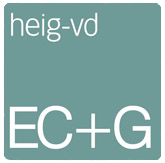
\includegraphics[width=0.75cm]{logoEC+G_163x165_ss_txt_ssBordBlanc.png}}

%%%%%%%%%%%%%%%%%%%%%%%%%%%%%%%%%%%%%%%%%%%%%%%%%%%%%%%%%

%\newcommand*\circled[1]{\tikz[baseline=(char.base)]{
%            \node[shape=circle,draw,inner sep=2pt] (char) {#1};}}
%\newcommand{\up}[1]{\textsuperscript{#1}}
\def\labelenumi{\theenumi}
%\setbeamertemplate{enumerate item}{\alph{enumi}}
%\setbeamertemplate{enumerate subitem}{\roman{enumii}.}
%\usepackage{outline}%
%\def\labeloutlni{\theoutlni}%
%\def\theoutlni{\alph{outlni}.}%
%\renewcommand{\labelenumi}{\alph{enumi}.)

\setbeamerfont{itemize/enumerate subbody}{size=\normalsize}
\setbeamerfont{itemize/enumerate subsubbody}{size=\normalsize}
\setbeamertemplate{itemize item}{-}
\setbeamertemplate{itemize subitem}{$\checkmark$}
\setbeamertemplate{itemize subsubitem}{$\blacktriangleleft$}

%\metroset{block=fill} %remplir les blocks

\makeatletter
\newcommand{\Pause}[1][]{\unless\ifmeasuring@\relax
\pause[#1]%
\fi}
\makeatother

%%%%%%%%%%%%%%%%%%%%%%%%%%%%%%%%%%%%%%%%%%%%%%%%%%%%%%%%%
\begin{document}

\frame{\titlepage}

\begin{comment}
\begin{frame}{Information}
    \warning \, Ce cours est destiné à des novices. Les fonctions et autres présentées dans ce document sont celles de bases. \\
    Si vous souhaitez aller plus loin, n'hésitez à regarder la documentation sur internet et les forums !
\end{frame}
\end{comment}

\begin{frame}{Table des matières}
  \setbeamertemplate{section in toc}[sections numbered]
  \tableofcontents%[hideallsubsections]
\end{frame}

%%%%%%%%%%%%%%%%%%%%%%%%%%%%%%%%%%%%%%%%%%%%%%%%%%%%%%%%%%%%%%%%%%%%%%%%%%%%%%%%%%%%%%%%%%%%%%%
\section{Introduction}
\begin{frame}{Introduction}
    \begin{table}
        \centering
        \begin{tabular}{c|c|c}
            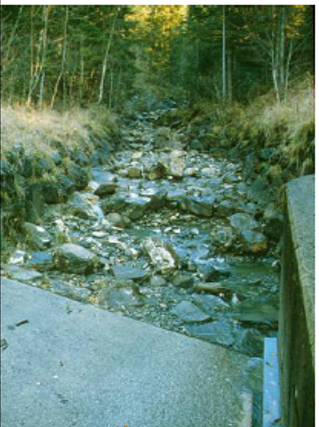
\includegraphics[height=3cm]{etiage.png} & 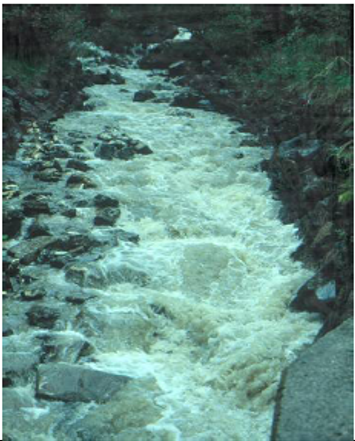
\includegraphics[height=3cm]{debitNormal.png} & 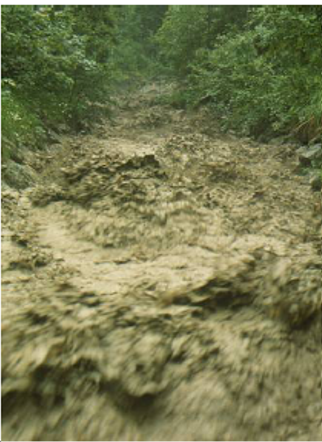
\includegraphics[height=3cm]{crue.png} \\
            \hline
            Étiage                & Débit normal           & Crue \\
            \textit{ou basse eau} & \textit{ou morphogène} &      \\       
            15 L/s                & 0.7 m\up{3}/s          & 10 m\up{3}/s \\
        \end{tabular}
    \end{table}
    \warning 1 m\up{3} = 1'000 L
\end{frame}

\begin{frame}{Veille hydrologique}
    \begin{figure}
        \centering
        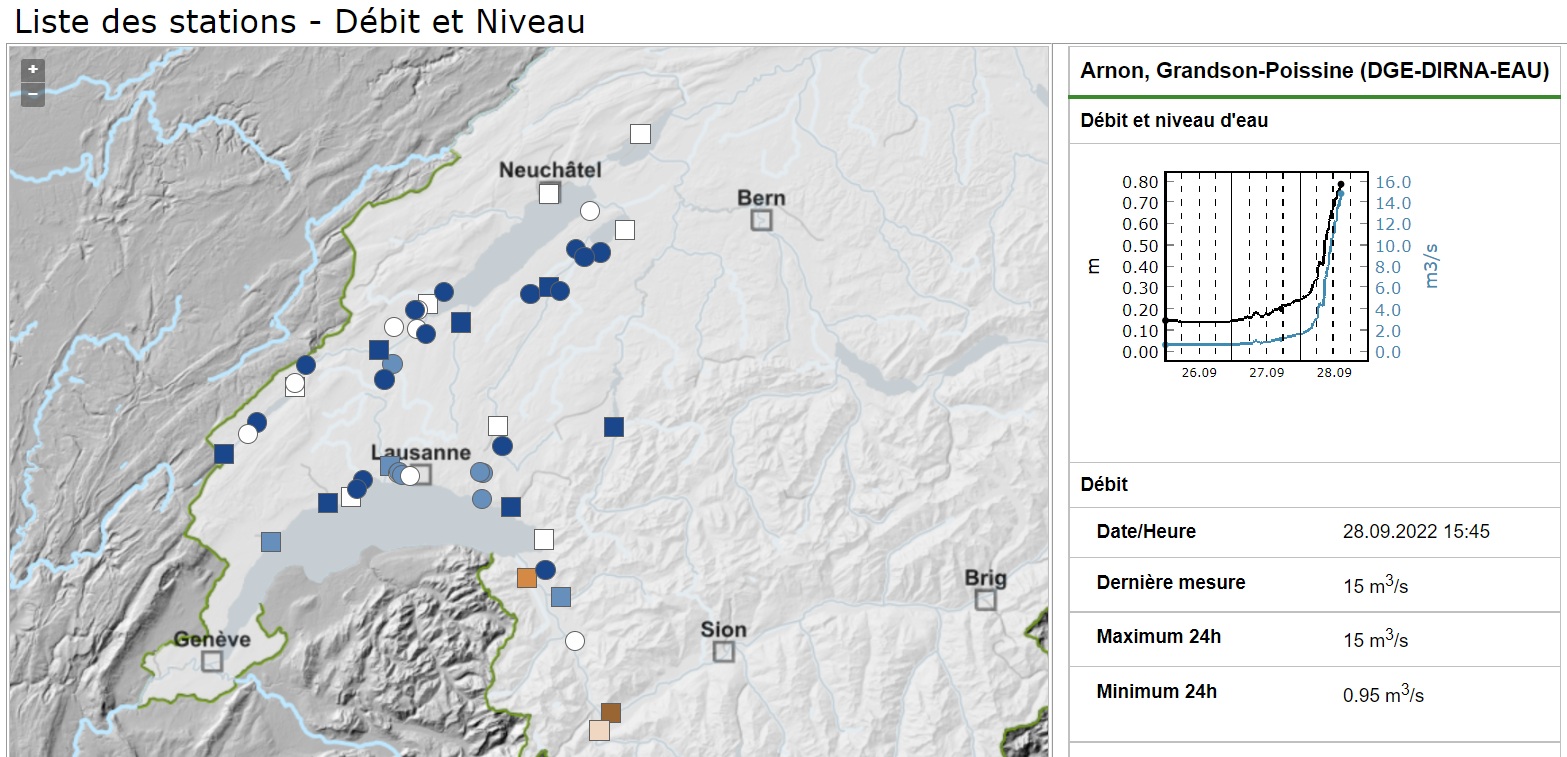
\includegraphics[width=8cm]{veilleHydrologique_VAUD.png}
        \caption{Capture d'écran du site internet \href{http://www.vhv.ch/}{http://www.vhv.ch/}}
    \end{figure}
    Une veille hydrologique est faite avec des stations pluviométriques, des stations sur les rivières (mesure débit et niveau), piézomètres, \dots
\end{frame}

\begin{frame}{Critères de dimensionnement}
    \begin{figure}
        \centering
        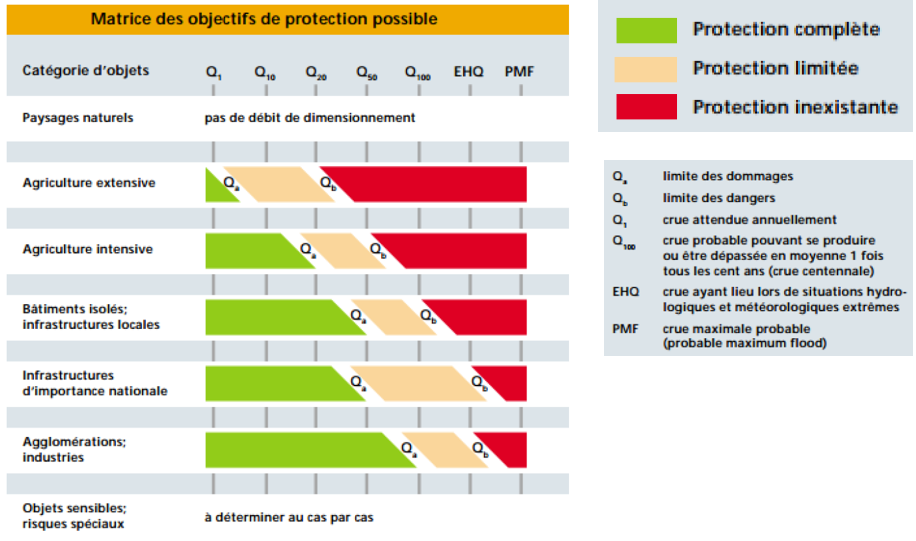
\includegraphics[width=8cm]{matriceObjectifsDimensionnement.png}
        \caption{Recommandations fédérales en matière de protection contre les crues. Selon les cas (communes, agglomérations, ...), on peut choisit le temps de retours et ainsi adapter les protections.}
    \end{figure}
\end{frame}

%%%%%%%%%%%%%%%%%%%%%%%%%%%%%%%%%%%%%%%%%%%%%%%%%%%%%%%%%%%%%%%%%%%%%%%%%%%%%%%%%%%%%%%%%%%%%%%
\section{Temps de retour}
\begin{frame}{Bases et principes}
    \begin{itemize}[label=$\rhd$]
        \item Crues moyennes : $T \in [2;5] \, \text{années}$
        \item Crues rares : $T \in \{10;30;100;300\}$ années et même plus selon les objectifs de protection
        \item Utilisation des données statistiques issues de la veille hydrologique \\
        $\implies$ Nous utilisons des données sur un certain temps et cela nous permettra d'extrapoler les débits pour des temps de retour de 30 à 300 ans.
    \end{itemize}
\end{frame}

\begin{frame}{Séparation des crues}
    \begin{figure}
        \centering
        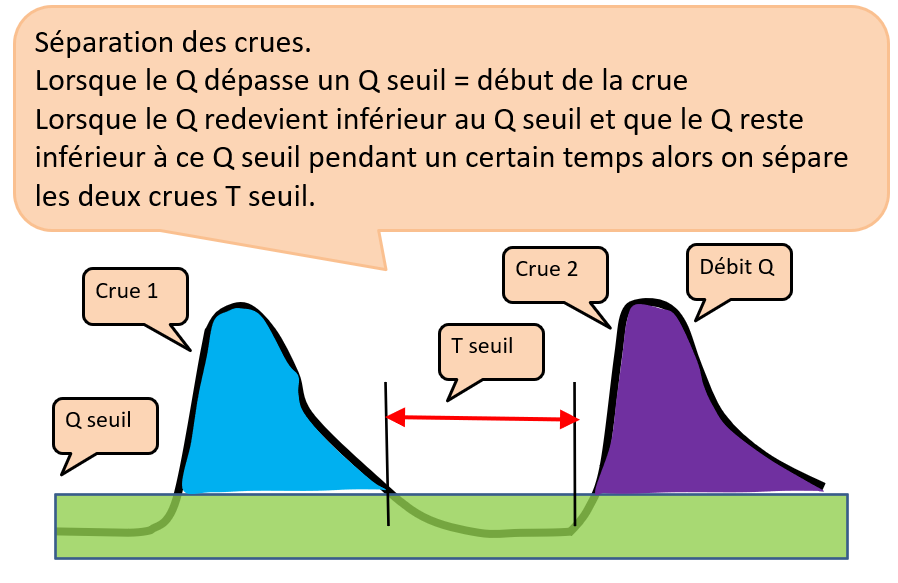
\includegraphics[width=8cm]{separationCrue.png}
    \end{figure}
\end{frame}

\begin{frame}{Marche à suivre pour calculer des temps de retour}
    \begin{enumerate}
        \item Vérification de \textbf{la stationnarité} des données statistiques
        \item Vérification de \textbf{l'homogénéité} des données statistiques
        \item Calcul des temps de retours $T$
        \item Calcul des paramètres de la \textit{loi de Gumbel} et de son débit $Q$
    \end{enumerate}
\end{frame}

\begin{frame}{1. Stationnarité}
    \begin{columns}
        \column{0.6\textwidth}
        \begin{figure}
            \centering
            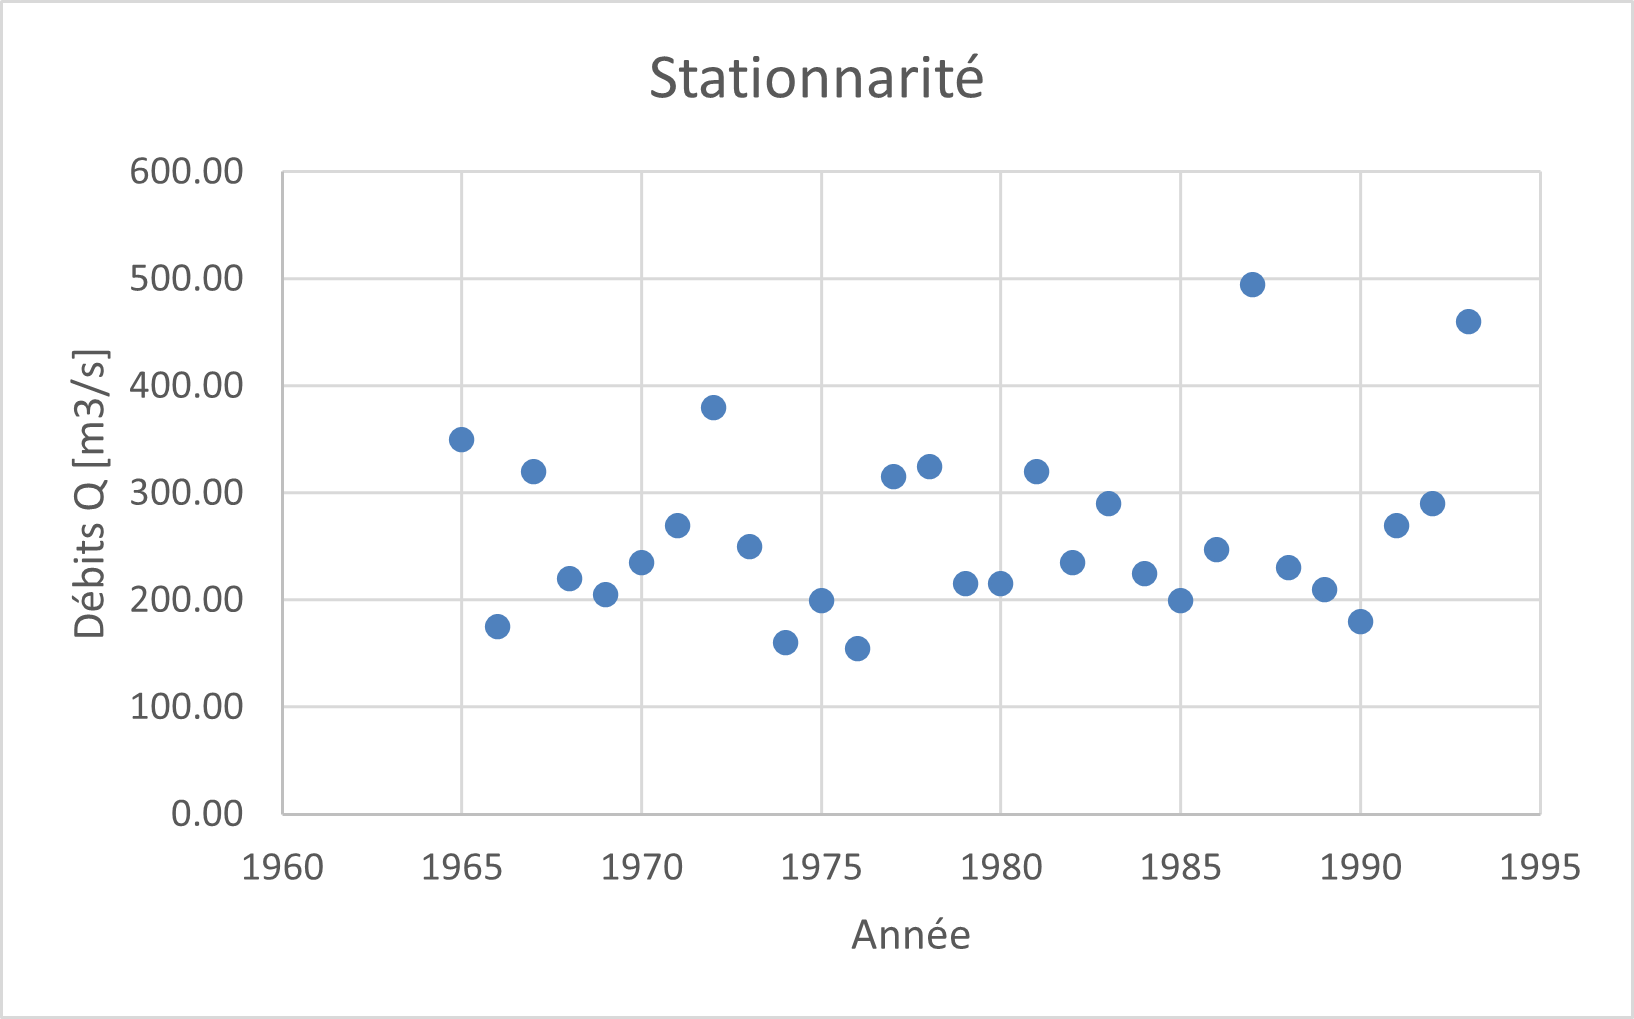
\includegraphics[width=5cm]{stationnarite.png}
        \end{figure}
        \column{0.4\textwidth}
        \begin{tabular}{c|c}
            \toprule
            \textbf{Année} & $\mathbf{Q_{max}}$ \\
            \midrule
            1965 & 350 \\
            1966 & 175 \\
            1967 & 320 \\
            1968 & 220 \\
            \dots & \dots \\
            \bottomrule
        \end{tabular}        
    \end{columns}
    \begin{exampleblock}{Nota}
        $\rightarrow$ Vérification que cela ne varie pas en fonction des années (courbe de tendance) \\
        $\rightarrow$ Visualiser l'évolution des crues de pointe en fonction des années donne un bon aperçu d'une dérive quelconque
      \end{exampleblock}
\end{frame}

\begin{frame}{2. Homogénéité}
    \begin{columns}
        \column{0.6\textwidth}
        \begin{figure}
            \centering
            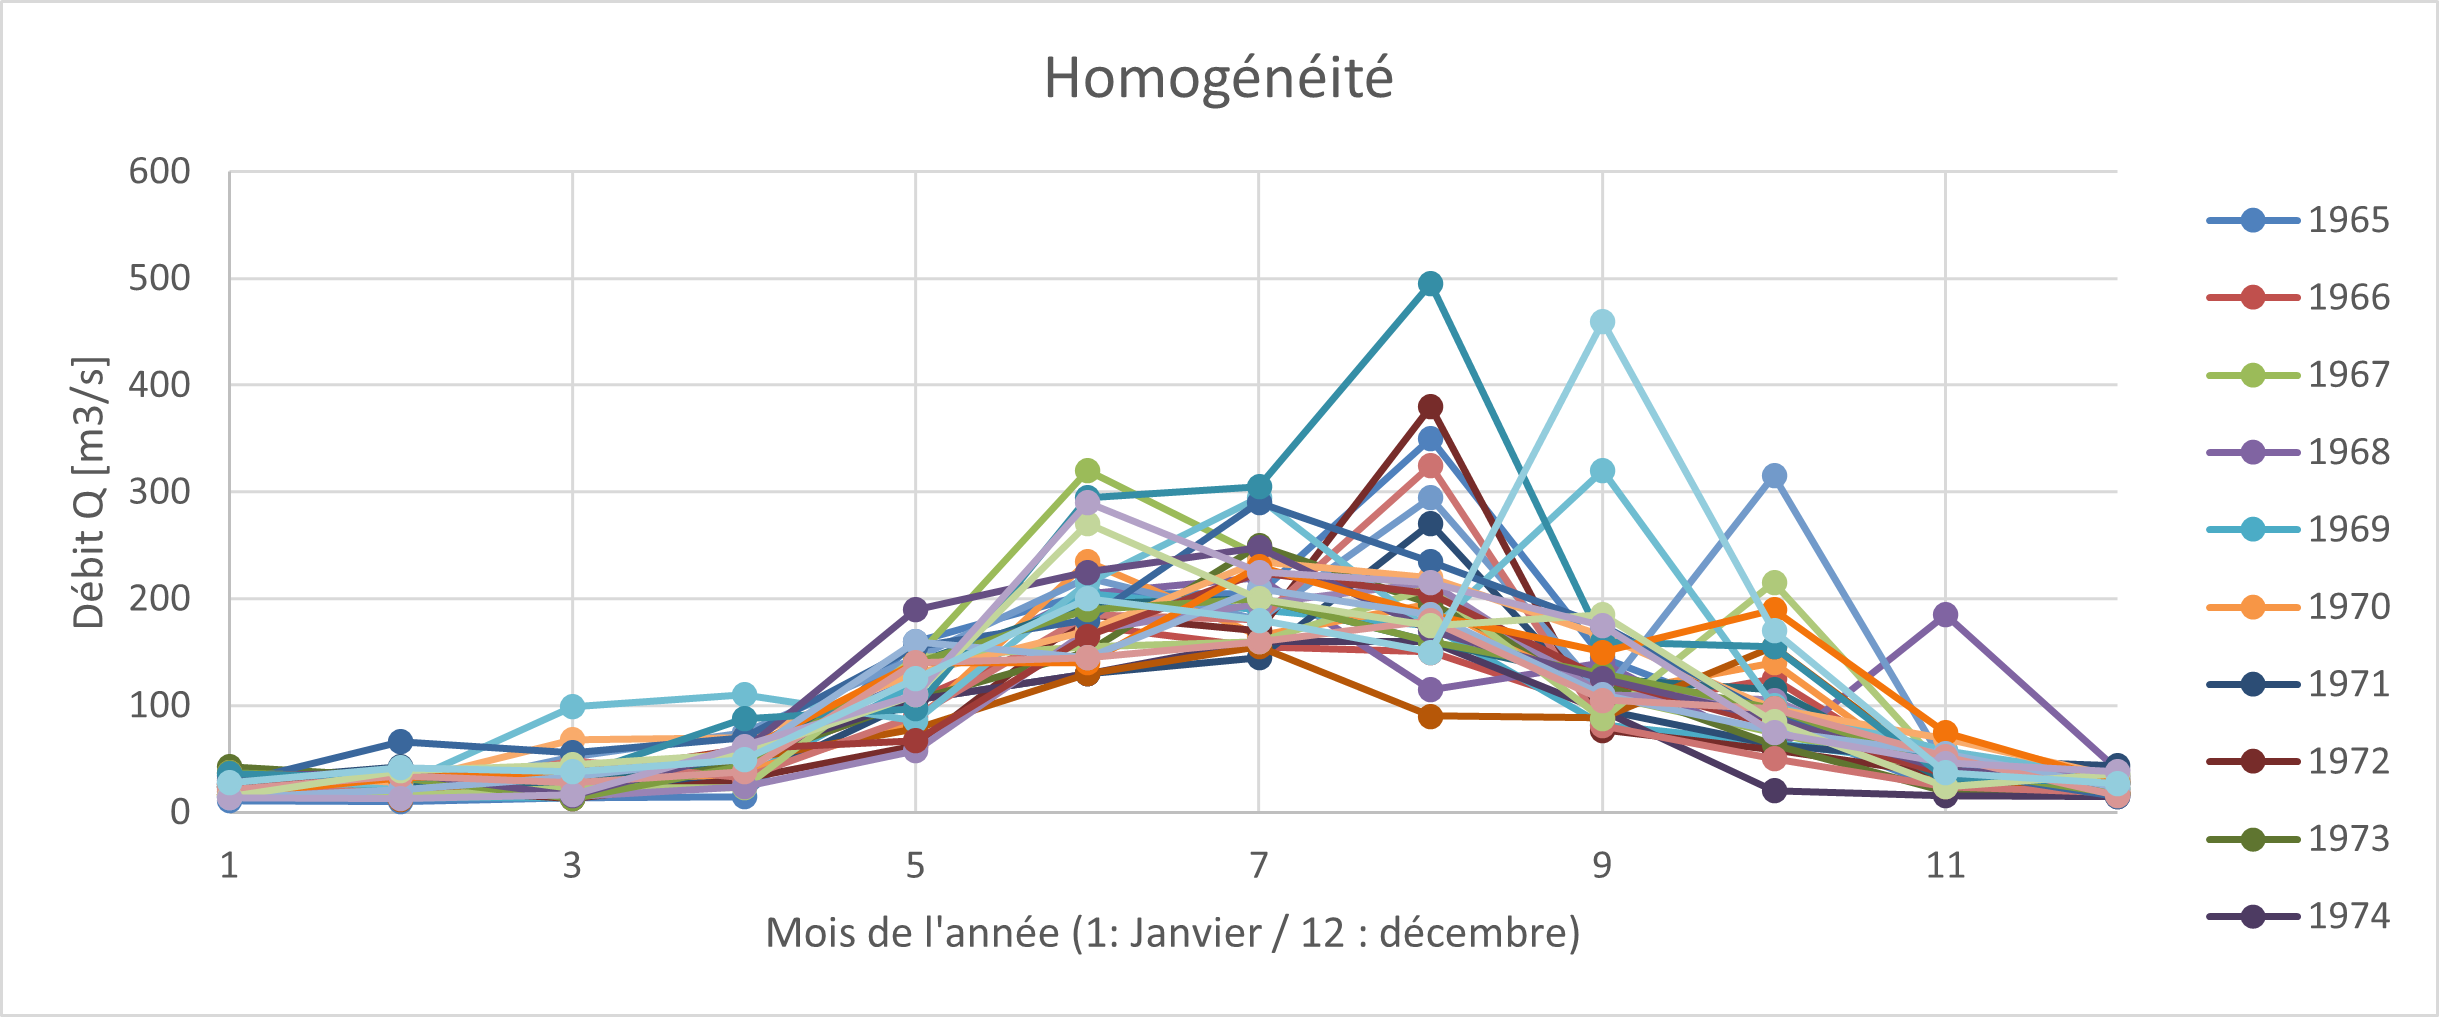
\includegraphics[width=5cm]{homogeneite.png}
        \end{figure}
        \column{0.4\textwidth}
        \begin{tabular}{c|c|c|c|c}
            \toprule
            \textbf{Année} & \textbf{Jan} & \textbf{Fev} & \textbf{Mar} & \textbf{\dots} \\
            \midrule
            1965  & 11.3  &  9.7  & 14.0  & \dots \\
            1966  & 16.6  & 18.5  & 16.6  & \dots \\ 
            1967  & 16.7  & 18.8  & 20.0  & \dots \\
            1968  & 19.2  & 14.6  & 21.0  & \dots \\
            \dots & \dots & \dots & \dots & \dots \\
            \bottomrule
        \end{tabular}        
    \end{columns}
\end{frame}

\begin{frame}{3. Temps de retour}
\end{frame}

\begin{frame}{4. Loi de Gumbel}
\end{frame}



\end{document}